\documentclass[inf, g]{pjatkThesis}


\usepackage{times}
\usepackage[polish]{babel}

\usepackage{graphicx}


\usepackage{makeidx}

\usepackage{lipsum}

\author{Patryk Ptasiński}
\album{10623}
\title{Nawigacja w warunkach miejskich przy użyciu danych o lokalizacjach sieci WIFI}
\type{inżynierska}
\supervisor{dr. inż Michał Tomaszewski}
\location{Warszawa}
\date{czerwiec 2017}

\begin{document}

\tableofcontents
%\listoffigures
%\listoftables

% zmiana nazwy abstraktu

\begin{abstract}
W swojej pracy przedstawię specyfikację technologi bezprzewodowej transmisji danych zwaną WIFI. Omówię problemy i wyzwania przy zbieraniu informacji o sieciach bezprzewodowych. Zanalizuję zebrane oraz publicznie dostępne dane o lokalizacjach sieci WiFi. 
\end{abstract}

\pagenumbering{arabic}
\baselineskip=22pt

\chapter*{Wprowadzenie}
\label{ch:wprowadz}

Skąd pomysł na badanie tematu sieci WiFi? Technologia ta już rozprzestrzeniła się na całym Świecie z ogromnym sukcesem. Więc można by postawić tezę, że w tym obszarze nie czeka na nas nic interesującego. Nic bardziej mylnego! Dopiero, teraz gdy sieci bezprzewodowe się rozprzestrzeniły na skalę masową, to możemy badać oraz projektować i tworzyć rozwiązania w oparciu na popularności tej technologii. Gdy wejdziemy do przeciętnego mieszkania wielopiętrowego bloku, to w zasięgu są dziesiątki, a czasem nawet setki bezprzewodowych sieci. Gdyby zapisać lokalizację tych wszystkich sieci bezprzewodowych, to utworzymy system, który umożliwia użytkownikom względne pozycjonowanie. W mojej pracy postaram się odpowiedzieć na pytanie, jak zbudować i korzystać z takiego systemu.

\chapter{Zagadnienia wykorzystania szablonu}

Ponieważ pisana praca inżynierska jest pracą techniczną, trzeba zachować pewne standardy techniczne charakterystyczne dla prac tego typu. Jednym z przykładów jest odwoływanie się do wszystkich:
\begin{itemize}
    \item obrazków,
    \item rysunków,
    \item schamatów,
    \item tabel,
    \item wykresów,
    \item \textit{itp}
\end{itemize}
Operację tę realizujemy z wykorzystaniem polecenia \texttt{\textbackslash ref}, i tak np gdy chcemy odwołać się do poniższego rysunku mówimy że: \textit{to i to zagadnienie jest ilustrowane przez rysunek \ref{fig:mobile}}. Możliwe są równie odwołanie się do konkretnego rozdziału, pod rozdziału czy punktu, np: \textit{ przykład wypunktowania alfabetycznego pokazano w podrozdziale \ref{ss:ex1}}.

Kolejnym bardzo ważnym elementem pracy technicznej jest wskazanie wszystkich źródeł jakie zostały wykorzystane w Państwa pracy. W tym przypadku wykorzystywany jest plik o rozszerzenie \texttt{.bib} oraz polecenie \texttt{\textbackslash cite} przykładowo odwołuję się do publikacji.\cite{Tomaszewski2000}


\begin{figure}[h!]
  \centering
    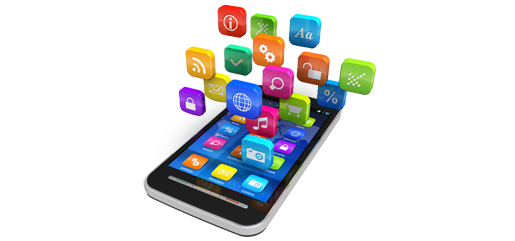
\includegraphics[width=0.5\textwidth]{images/mobile-banner}
  \caption{Close-up of a gull}
  \label{fig:mobile}
\end{figure}

\lipsum[1]

\section{Structure}
\lipsum[2]

\subsection{Top Matter}
\lipsum[1]

\subsubsection{Wypunktowanie}
\label{ss:ex1}

Przykład wypunktowania:

\begin{description}
	\item[(a)] minimalizacja liczby niezależnych parametrów funkcji plenoptycznej;
	\item[(b)] identyfikacja schematu próbkowania plenoptycznego w modelu kamery otworkowej;
	\item[(c)] identyfikacja ruchu wykonywanego przez element plenoptyczny;
	\item[(d)] filtracja funkcji plenoptycznej w systemach percepcji wizualnej.
\end{description}
\lipsum[1]

\section{Minimalizacja parametrów funkcji plenoptycznej}
\label{sec:mpfp}
\chapter{Wytwarzanie oprogramowania}
%TODO:

\section{Wersjonowanie}
%TODO:
Git - wersjonowanie (i dlaczego Github?).

\section{Projektowanie}
%TODO:
Projektowanie (wybór technologii, architektury).



\chapter{Analiza problemu}
Dostep do internetu - posiadanie na telefonie bazy danych wszystkich lokalizacji sieci wifi jest dosyć nierealistyczne ponieważ rozmiar danych dla warszawy to byłoby około 40MB danych przedstawionych w formacie CSV lub 9MB dla spakowanego archiwum tych danych. Dodaktowo dochodzi element obliczania lokalizacji na tak rozległych danych. Gdy natomiast, wziąć pod uwagę bazę stacji GSM. To taka baza jest dużo mniejsza, oraz jej dane nie zmieniają się tak często. Taką bazę można umieszczać na urządzeniach by ustalały lokalizację w sposób stuprocentowy offline i anonimowo. Niestety lokalizacja na podstawie puntków stacji GSM jest niedokładna. Średnia dokładność dla lokalizacji ustalonej na bazie nadajników GSM to 3000m. Gdzie dla sieci wifi to 30m

%TODO? jakieś źródła tych dokładności lokalizacji by się przydały. Np. na podstawie 

Podczas gdy użytkownik ma dostęp do internetu, to można go zlokalizować na podstawie adresu ip. Podanych sieci wifi które ma w zasięgu. Podanych stacji GSM które ma w zasięgu.

%TODO: Skompresowane dane do lokalizowania się w Warszawie? Czy możliwe jest zapisanie lokalizacji sieci wifi w taki sposób aby zajmowały mało miejsca, nie były kosztowne do obliczenia, offline?
\section{Przetwarzanie danych osobowych}


\section{Lokalizacja sieci wifi a wpa.darkircop.org}
Na stronie wpa.darkircop.org możemy znaleźć 


\chapter{Backend}

Ze względu na ogrom informacji i potrzebę istnienia miejsca w którym połączymy lokalizację punktów dostępów z ich identyfikatorami zdecydowałem się na stworzenie aplikacji serwerowej. 

\section{Technologia}

Ze względu na moje doświadczenie przy pracy z technologią Ruby on Rails, właśnie to rozwiązanie zostało wybrane.

Możliwe alternatywy:
 - C Sharp - MVC
 - PHP
 - Node.js (+ Express)
 - Java
 - Python Django

Baza danych : postgres

Alternatywy:
 - SQLite
 - MySQL
 - MSSQL
 - Mongodb
 
 
\subsection{MVC}
Opisanie wzorca architektoniczego MVC

\subsection{CRUD - REST/SOAP}

\subsection{JSON/HTML}

\subsection{Stack technolgoiczny}
Coś o dockerze(ngnix proxy). Coś o azure. Dlaczego Cloudflare?

% może jakieś screenshoty z panelu azure?

\section{Implementacja}

Implementację rozpocząłem od importu istniejących danych o lokalizacjach sieci wifi z różnych serwisów.

\subsection{Istniejące dane}

Cztery serwisy udostępniają dumpy bazy, ich nazwy razem z rozmiarem spakowanych danych które udostępniają:
 - openwifi.su (openwlanmap.org) - 245,7MB - CSV spakowany do tar.bz2
 - radiocells.org (openbmap) - 1.6GB - baza danych sqlite
 - mylnikov.org - 657 MB - CSV spakowany do zip

\subsection{Import danych i denormalizacja}
Ze względu na prędkość importu zdecydowałem się zdenormalizować w tabeli obserwacji punktów dostępów, kolumnę BSSID - opisującą adres sprzętowy urządzenia. Dzięki temu mogłem użyć biblioteki activerecord-import. Która pozwala na import danych do bazy danych poprzez bardzo przyjemny interfejs.

\subsubsection{Dane z mylnikov.org}

Na samej stronie, twórca twierdzi, że jego baza danych jest kompilacją baz openBmap.orb oraz OpenWIFI.su

\subsection{WifiObservation}
Jako formę reprezentacyjną danych utworzyłem model WifiObservation z następującymi kolumnami:

Do aplikacji dodałem dwa widoki: Mapa obserwacji oraz mapa "ciepła" - która pokazuje zagęszczenie zbadanych sieci wifi.

\subsection{GeoJSON}
%FeatureCollection
Przy mapie obserwacji aby zapresentować dane z bazy wybrałem standard GeoJSON. 

\begin{lstlisting}[caption=Ruby geojson\_hash]
  def geojson_hash
    {
      type: 'Feature',
      geometry: {
        type: 'Point',
        coordinates: geojson_coordinates
      },
      properties: {
        id: id,
        bssid: bssid
      }
    }
  end
\end{lstlisting}

Niestety przy generowaniu pięćdziesięciu tysięcy obserwacji punktów dostępów, serwer Railsowy wykonywał dużo przetwarzania danych, co skutkowało bardzo długim czasem odpowiedzi - około dziesięciu sekund.

\subsubsection{Benchmark}

Pomyślałem, że możliwym przyspieszeniem będzie przeniesienie generowania struktury GeoJSON do bazy danych.

\begin{lstlisting}[caption=Ruby geojson\_hash]
SELECT json_build_object(
    'type',       'Feature',
    'id',         gid,
    'geometry',   ST_AsGeoJSON(geom)::json,
    'properties', json_build_object(
        'feat_type', feat_type,
        'feat_area', ST_Area(geom)::geography
     )
) FROM input_table;
\end{lstlisting}

Niestety, nie zauważyłem różnicy między jednym a drugim rozwiązaniem.

%tutaj wynik z benchmarku

Postanowiłem optymalizować w innych obszarach. Dużym zaskoczeniem było dla mnie, użycie metody to_json na kolekcji przygotowanych danych. Czas odpowiedzi z dziesięciu tysięcy milisekund spadł do czterech tysięcy milisekund dla pięćdziesięciu tysięcy rekordów.


To przywiodło mi na myśl, że byłby to idealny moment na sprawdzenie wydajności między różnymi wersjami Rubiego. Projekt na początku utworzyłem na wersji 2.3.3 ze względu na wcześniej przygotowany szablon aplikacji. Stwierdziłem że sprawdzę nowszą wersję - 2.4.1 - oraz konkurującego odpowiednika jruby - 9

\begin{lstlisting}[caption=Benchmark geojson]
Benchmark.bm do |x|
  x.report('JSON[pluck_geojson]') { 5.times { JSON[WifiObservation.limit(50_000).pluck_geojson] }}
  x.report('pluck_geojson.to_json') { 5.times {  WifiObservation.limit(50_000).pluck_geojson.to_json }}
  x.report('JSON[map(&:geojson_hash)]') { 5.times {  JSON[WifiObservation.limit(50_000).map(&:geojson_hash)] }}
  x.report('map(&:geojson_hash).to_json') { 5.times {  WifiObservation.limit(50_000).map(&:geojson_hash).to_json }}
end
\end{lstlisting}

Ruby 2.3.3:

       user     system      total        real
JSON[pluck_geojson]  7.970000   0.300000   8.270000 ( 15.635793)
pluck_geojson.to_json 29.620000   0.630000  30.250000 ( 38.220882)
JSON[map(&:geojson_hash)] 16.530000   0.510000  17.040000 ( 19.063228)
map(&:geojson_hash).to_json 38.970000   1.240000  40.210000 ( 43.482492)

Ruby 2.4.1:
       user     system      total        real
JSON[pluck_geojson]  7.760000   0.270000   8.030000 ( 15.252685)
pluck_geojson.to_json 30.350000   0.680000  31.030000 ( 38.310567)
JSON[map(&:geojson_hash)] 15.190000   0.410000  15.600000 ( 17.504994)
map(&:geojson_hash).to_json 38.660000   0.940000  39.600000 ( 42.145208)

jruby-9.1.9.0:
       user     system      total        real
JSON[pluck_geojson]  2.040000   0.170000   2.210000 (  8.073360)
pluck_geojson.to_json  5.780000   0.220000   6.000000 ( 10.977538)
JSON[map(&:geojson_hash)] 74.390000   0.850000  75.240000 ( 32.687321)
map(&:geojson_hash).to_jsonJava::JavaLang::OutOfMemoryError: GC overhead limit exceeded


\subsubsection{Klastrowanie markerów}

Dodatkowym problemem z jakim się spotkałem, to czytelność i jednocześnie wydajność prezentacji dziesięciu tysiecy punktów na w kontrolce map'owej leaflet. Bez użycia klastrowania znaczników, Firefox zawieszał się na ponad 20 sekund, aby wyrysować wszystkie punkty na mapie.


%Ze względu na wielkość importowanych danych i ograniczoną wydajność, ograniczyłem import danych do koorydynatów goeograficznych... 
%\subsubsection{Geografia}
%Zakres ten obejmuje X kilometrów kwadratowych. Można opisać, dla uproszczenia że obszar ten na północnym zachodzie kończy się na ..., na północnych wschodzie na ..., na południowym wschodzie na ... oraz na południowym zachodzie na ...

%TODO: obrazek z wizualizacją granic 


%Po zaimportowaniu danych zrobiłem analizę i zauważyłem, że dane pomiędzy tymi bazami nie są unikalne czego można było się akurat spodziewać. Jednak, że dane w ramach jednej bazy danych też się powtarzają.


% https://static.googleusercontent.com/media/www.google.com/pl//googleblogs/pdfs/google_submission_dpas_wifi_collection.pdf



\subsection{Geolokacja - Location Provider}
% https://developers.google.com/maps/documentation/geolocation/intro
% https://radiocells.org/geolocation
% https://www.ghacks.net/2014/02/03/switch-googles-location-service-mozillas-firefox/

\chapter{Android}
\section{Bezpieczeństwo i anonimowość użytkownika}
\subsection{Uprawnienia na Android}
%TODO: opisać nowy system uprawnień na Androidzie

Począwszy od Androida 6.0 (poziom API 23) użytkownicy przyznają uprawnienia do aplikacji podczas uruchamiania aplikacji, a nie podczas instalowania aplikacji. To podejście usprawnia proces instalacji aplikacji, ponieważ użytkownik nie musi przyznać uprawnień podczas instalowania lub aktualizowania aplikacji. Daje to również użytkownikowi większą kontrolę nad funkcjonalnością aplikacji; Na przykład użytkownik może zdecydować się udostępnić kamerę dostęp do aparatu, ale nie do lokalizacji urządzenia. Użytkownik może cofnąć uprawnienia w dowolnym momencie, przechodząc do ekranu Ustawienia aplikacji.\cite{NewPermissionsModelInAndroid60}

\subsection{Uprawnienie do WIFI bez GPS}
Dla użytkowników smartfonów, którym zależy na anonimowości i prywatności proces lokalizowania na podstawie sieci WIFI może być mało podejrzany.

W przypadku w którym dana aplikacja korzysta tylko z uprawnień do stanu WIFI, może to ukryć prawdziwe zamiary aplikacji. Użytkownik widząc, że aplikacja nie korzysta z uprawnień do lokalizacji, założy, że jego pozycja nie będzie ujawniona - co w rzeczywistości, bedzie nieprawdą.

Dodatkowo w nowej wersji Androida, nawet jeżeli użytkownik jest świadom, że aplikacja może go lokalizować na podstawie sieci wifi. To wyłączenie samego modułu WiFi w telefonie, jest niesktuczene, bo można skanować w poszukiwaniu sieci wifi gdy moduł jest wyłączony z perspektywy użytkownika.

Posiadanie informacji o sieciach do których telefon jest podłączony jest jeszcze bardziej groźne niż sama lokalizacja uzytkownika. Można szacować w jakiej firme użytkownik pracuje na podstawie tego, że smartfon był połączony z daną siecią wifi przez 8 godzin dnia pracy, od 9 do 17. Dodatkowo firmy zazwyczaj mają swoją nazwę ustawioną jako SSID punktu dostępu do swoich sieci. Dodatkowo można lokalizować użytkownika w jego domu, wiedząc do jakiej sieci się łączy w przez resztę dnia (i nocy). To można wstępnie określić że mieszka w danym bloku. A znając adres MAC, można dokładnie określić mieszkanie w którym dana sieć wifi pracuje poprzez przejście z odpowiednim skanerem przez budynek. 

%TODO sprawdzić czy jestem w stanie dostać adres MAC urządzenia Android na którym jest aplikacja zainstalowana.
Taki skaner mogłby też pokazać czy dane urządzenie jest połączone do sieci, tym samym stwierdzając czy dany użytkownik jest w swoim mieszkaniu czy nie (choć również ta informacja jest dostępna poprzez samą aplikację mobilną).


\chapter{Szkic kolejnych rozdziałów}
Jak często jest w stanie Android skanować w poszukiwaniu WIFI?

Dokładność ostatniej pozycji GPS w metrach

Zmierzona wartość + estymacja vs rzeczywiste położenie punktu dostępowego

Problem tej pracy składa się z dwóch części:
 - Zbieranie i przetwarzanie danych
 - Lokalizowanie użytkownika na podstawie bazy danych lokalizacji punktów dostępu.
 
Sam problem zbierania danych też składa się z wielu części:
 - częstotliwość odświeżania koordynatów GPS
 - częstotliwość odświeżania sieci WIFI w zasięgu
 - zbieranie danych w budynkach, tunelach i innych miejsach o ograniczonym dostępie do GPS.
 

Źródła lokalizacji sieci wifi - https:\/\/en.wikipedia.org\/wiki\/Wi-Fi\_positioning\_system

Rozmiar baz danych z informacjami o lokalizacji sieci wifi

Powody do lokalizowania bez gps:
 - laptopy nie mają gps
 - szybsze określenie pierwszej lokalizacji wifi
 - mniejsze zuużycie energii
 
Zasięg i lokalizowanie. 5GHz vs 2GHz

Wizualizacja rozproszenia sygnału wifi
https://jasmcole.com/2014/08/25/helmhurts/
The Helmholtz equation
This gif is a particular case of wave propagation. Only one frequency. And the materials of the walls are idealized, which inherently is inaccurate. In reality, the permeability of common household materials is hard to find and varies with frequency. The source is also idealized as a point source, not a monopole. And, iirc the reflections are not accounted for. 


Wyrzucac accespointy ktore sa telefonami/androidami/iosami ale tez Huawei MiFi

Aplikacja Android

    Co wiadomo o sieci Wifi w Androidzie? klasa ScanResult (rzeczywistość na przykładzie Nexus 5 + dokumentacja)
    Jak szybko można skanować sieci Wifi w Androidzie? * Moreover, you still need to scan the 12 Wi-fi channels to be sure that you are detecting all access points. An access point broadcasts a beacon every 100ms * 12 channels = 1.2 seconds. Spending less time than that and you risk missing access points. (z http://stackoverflow.com/questions/9533476/increasing-wifi-scan-rate)
    
Location provider: https:\/\/www.radiocells.org\/geolocation



Bazy danych

    Porównanie ile jest zmapowanych sieci w Warszawie do np innych miast?
    Porównanie ile sieci zostało wykorzystanych z całej puli?
    Porównanie jak często dumpy mają powtarzające się dane?


Aplikacja Railsowa

    Problemy z serializacją obiektów (WifiService) w Railsach (wydajnościowe)
    Sposób przetrworzenia i serwowania danych dla heatmapy
    Problemy struktury przechowywania i przetwarzania danych na serwer
    Problem lokalizowania accesspointa na podstawie posiadanych danych (obrazki), mapowanie korzystając z jednego odbiornika na podstawie zmiany sygnału na zaznaczonej trasie
        Proste mapowanie
        Srednie
        Moje
    Development aplikacji androidowej na podstawie fork'a z opracowanej od dawna aplikacji i podobnych wymaganiach funkcjonalnych (raczej nie)


Apliakacja Androidowa

    Android Studio v2.3.1
    Gradle 2.1.3
    com.michaelpardo:activeandroid:3.1.0

Wybrałem bibliotekę ActiveAndroid jako element Object-Relational Mapping (ORM) ze względu na swoje podobieństwo do ActiveRecord ze świata języka programowania Ruby oraz ze względu na użycie bazy SQLite która jest popularnym rozwiązaniem na Androidzie.

Lista wersji androida sdk i popularny kod.

W pierwszym etapie, skupiłem się na skanowaniu wifi oraz na pracy z (Klasa skanująca) oraz ScanResult z pakietu wifi. Zastosowałem prosty linear layout w wersji horyzontalnej. Gdy już miałem wyniki skanowania, to stwierdziłem że trzeba je zapisać w bazie danych korzystając z biblioteki ActiveAndroid. Gdy już skanowanie oraz zapis do bazy danych mamy z głowy, to możemy przejść do bieżącej lokalizacji. W tej kwestii skorzystałem z SmartLocation w trybie pracy Navigate oraz continious. Trzeba pamiętać że takie ustawienie jest niekorzystne dla czasu pracy na baterii. Dodatkowo do widoku LinearLayout dodałem flagę "android wake lock flag" żeby ekran nie usypiał się.

W kolejnym etapie aplikacji mobilnej można się skupić na dodaniu:

    widoku mapy
    przeniesieniu skanowania wifi do BackgroundService

W tym momencie możemy śmiało zakończyć etap pierwszy. W etapie drugim skupię się na przekazaniu danych do serwera. Etap drugi możemy podzielić na następujące punkty:

    ustalenie formatu przekazywanych danych
    zmodyfikowanie modelu WifiObservation poprzez dodanie flagi exported
    utworzenie odpowiednich akcji i widoków w aplikacji mobilnej (konfigurowalny url serwera, przycisk do exportu)
    możliwość usuwania wyexportowanych danych (oszczędność miejsca na urządzeniu)
    przyjęcie przekazanych danych na serwerze rails.

Denormalizacja danych

Ze względu na cechę badawczą pracy oraz na proste podejście do problemu, zdecydowałem się na zdenormalizowanie danych w bazie danych aplikacji mobilnej.

Dane zdenormalizowane będą zajmować więcej miejsca ale umożliwą na dokładniejsze lokalizowanie miejsca w którym jest ustawiony accesspoint.

Wszystkie dane będą zapisane w pojedyńczej tabeli. Problem jaki powstaje poprzez taki stan schematu bazy danych jest to, żeby znaleźć, które sieci wifi były znalezione w konkretnym skanie, trzeba szukać sieci o takiej samej wartości seen\_at.

przetwarzanie danych osobowych ( w ameryce nielegalne jest zbieranie ssid)


WARDriving!

korelacja nazwy sieci wifi do firm znajdujacych sie w poblizu (todo: znajdz baze danych firm w warszawie)

lokalizacja wiekszosci sieci wifi w publicznych bazach danych znajduje sie "na ulicy" ze względu na metodologię skanowania.
problem: jak stwierdzić czy sieć wifi znajduje się po lewej stronie ulicy czy po prawej.
\chapter*{Słownik pojęć}

\newcommand{\entry}[2]{\textbf{#1}\ $\bullet$\ {#2}}

\entry{ORM}{skrótowe oznaczenie dla "mapowanie obiektowo-relacyjne" (od angielskiego Object-Relational Mapping).}

\entry{Punkt dostępu (od ang. Accesspoint)}{Stacja bazowa WIFI.}
\entry{Aplikacja internetowa}{Aplikacja WWW/HTTP (webowa)}
\entry{SSID}{Nazwa punktu dostępu}
\entry{BSSID}{Mac Address}
\entry{Interfejs}{Międzymordzie}
\entry{Klastrowanie}{Zadaniem klastrowania jest pogrupowanie zbioru obserwacji w klastry tak, aby w ramach klastra obserwacje były do siebie jak najbardziej podobne, a jednocześnie jak najbardziej różne od obserwacji w innych klastrach.}
%https://eduwiki.wmi.amu.edu.pl/klastrowanie

\entry{Kanał (w kontekście sieci przezprzewodowych i punktów dostępów)}{WIFI operuje na określonych częstotliwościach. W przypadku 802.11g jest ich 14. Te poszczególne częstotliwości nazywamy kanałami.}

\entry{wardriving}{"zbieranie" jak najwiekszej ilosci sieci wifi.}
%https://en.wikipedia.org/wiki/Wardriving

\entry{MIMO (od ang. Multiple-Input-Multiple-Output)}{rozwiązanie w którym karta sieciowa posiada wiele wyjść i wiele wejść, przez co można nadawać i odbierać na specyficznym Wejściu/Wyjściu które posiada lepsze parametry komunikacji}

\entry{denormalizacja}{jest to wprowadzenie kontrolowanej nadmierności do bazy danych w celu przyśpieszenia wykonywania na niej operacji (np. obsługiwania zapytań); dzięki denormalizacji bazy unika się kosztownych operacji połączeń tabel}
%https://pl.wikipedia.org/wiki/Denormalizacja_bazy_danych




%\addcontentsline{toc}{chapter}{Literatura}

\bibliographystyle{abbrv}
\bibliography{bibliografia}
    
\end{document}